The user interface is constructed from a hierarchy of reusable React components, following a component-based architecture. This modular approach was facilitated by two main libraries: \texttt{shadcn/ui} and \texttt{@assistant-ui/react}.

For the main application shell and dashboard views, \texttt{shadcn/ui} was used extensively. This library provides a set of styled, accessible, and composable components that serve as the foundational building blocks. The interface is wrapped by a sidebar with navigation links to the main sections of the platform, such as ``Agent Hub'', ``Open Chat'', and ``Create Agent'' (as well as an ``\acs{api} Documentation'' external link). The lower section of the sidebar contains a menu for the user profile, to reset their password, see their access key for the documentation page, and log out. The dashboard also includes a header on top of the page, with a button to toggle the sidebar, breadcrumbs to aid in the navigation, and three icon menus on the right side: one for \acs{llm} selection, one for language selection, and another for theme selection (dark, light or system mode).

The platform includes several forms for authentication, password reset, and agent creation. These forms utilize \texttt{shadcn/ui}'s form components, which are built on top of \texttt{react-hook-form} for efficient form state management. Validation was implemented using \texttt{Zod} \cite{ZOD}, a TypeScript-first schema declaration and validation library, ensuring that all user inputs have correct values before being processed.

The main \texttt{AgentHub} view features the \texttt{AgentCard} component, which is built by composing \texttt{shadcn/ui}'s \texttt{Card}, \texttt{Button}, and \texttt{Tooltip} components to create a custom \acs{ui} element. These cards are then orchestrated within a grid display of agents in the view, which provides a comprehensive dashboard for browsing, searching, and managing all available recommender agents, as shown in Figure~\ref{FIG:AGENT_HUB}.

To enhance usability, the state of the Agent Hub's search, filter and paging controls is persisted in the URL's query parameters. This implementation allows users to bookmark a specific filtered view or share a direct link to it with others, ensuring a consistent and reproducible experience. Each search query is also debounced to prevent excessive query requests. Additionally, all searching, filtering and paging operations are executed as database queries, ensuring scalable and efficient retrieval.

\begin{figure}[Agent Hub]{FIG:AGENT_HUB}{The Agent Hub, the platform's main dashboard.}
    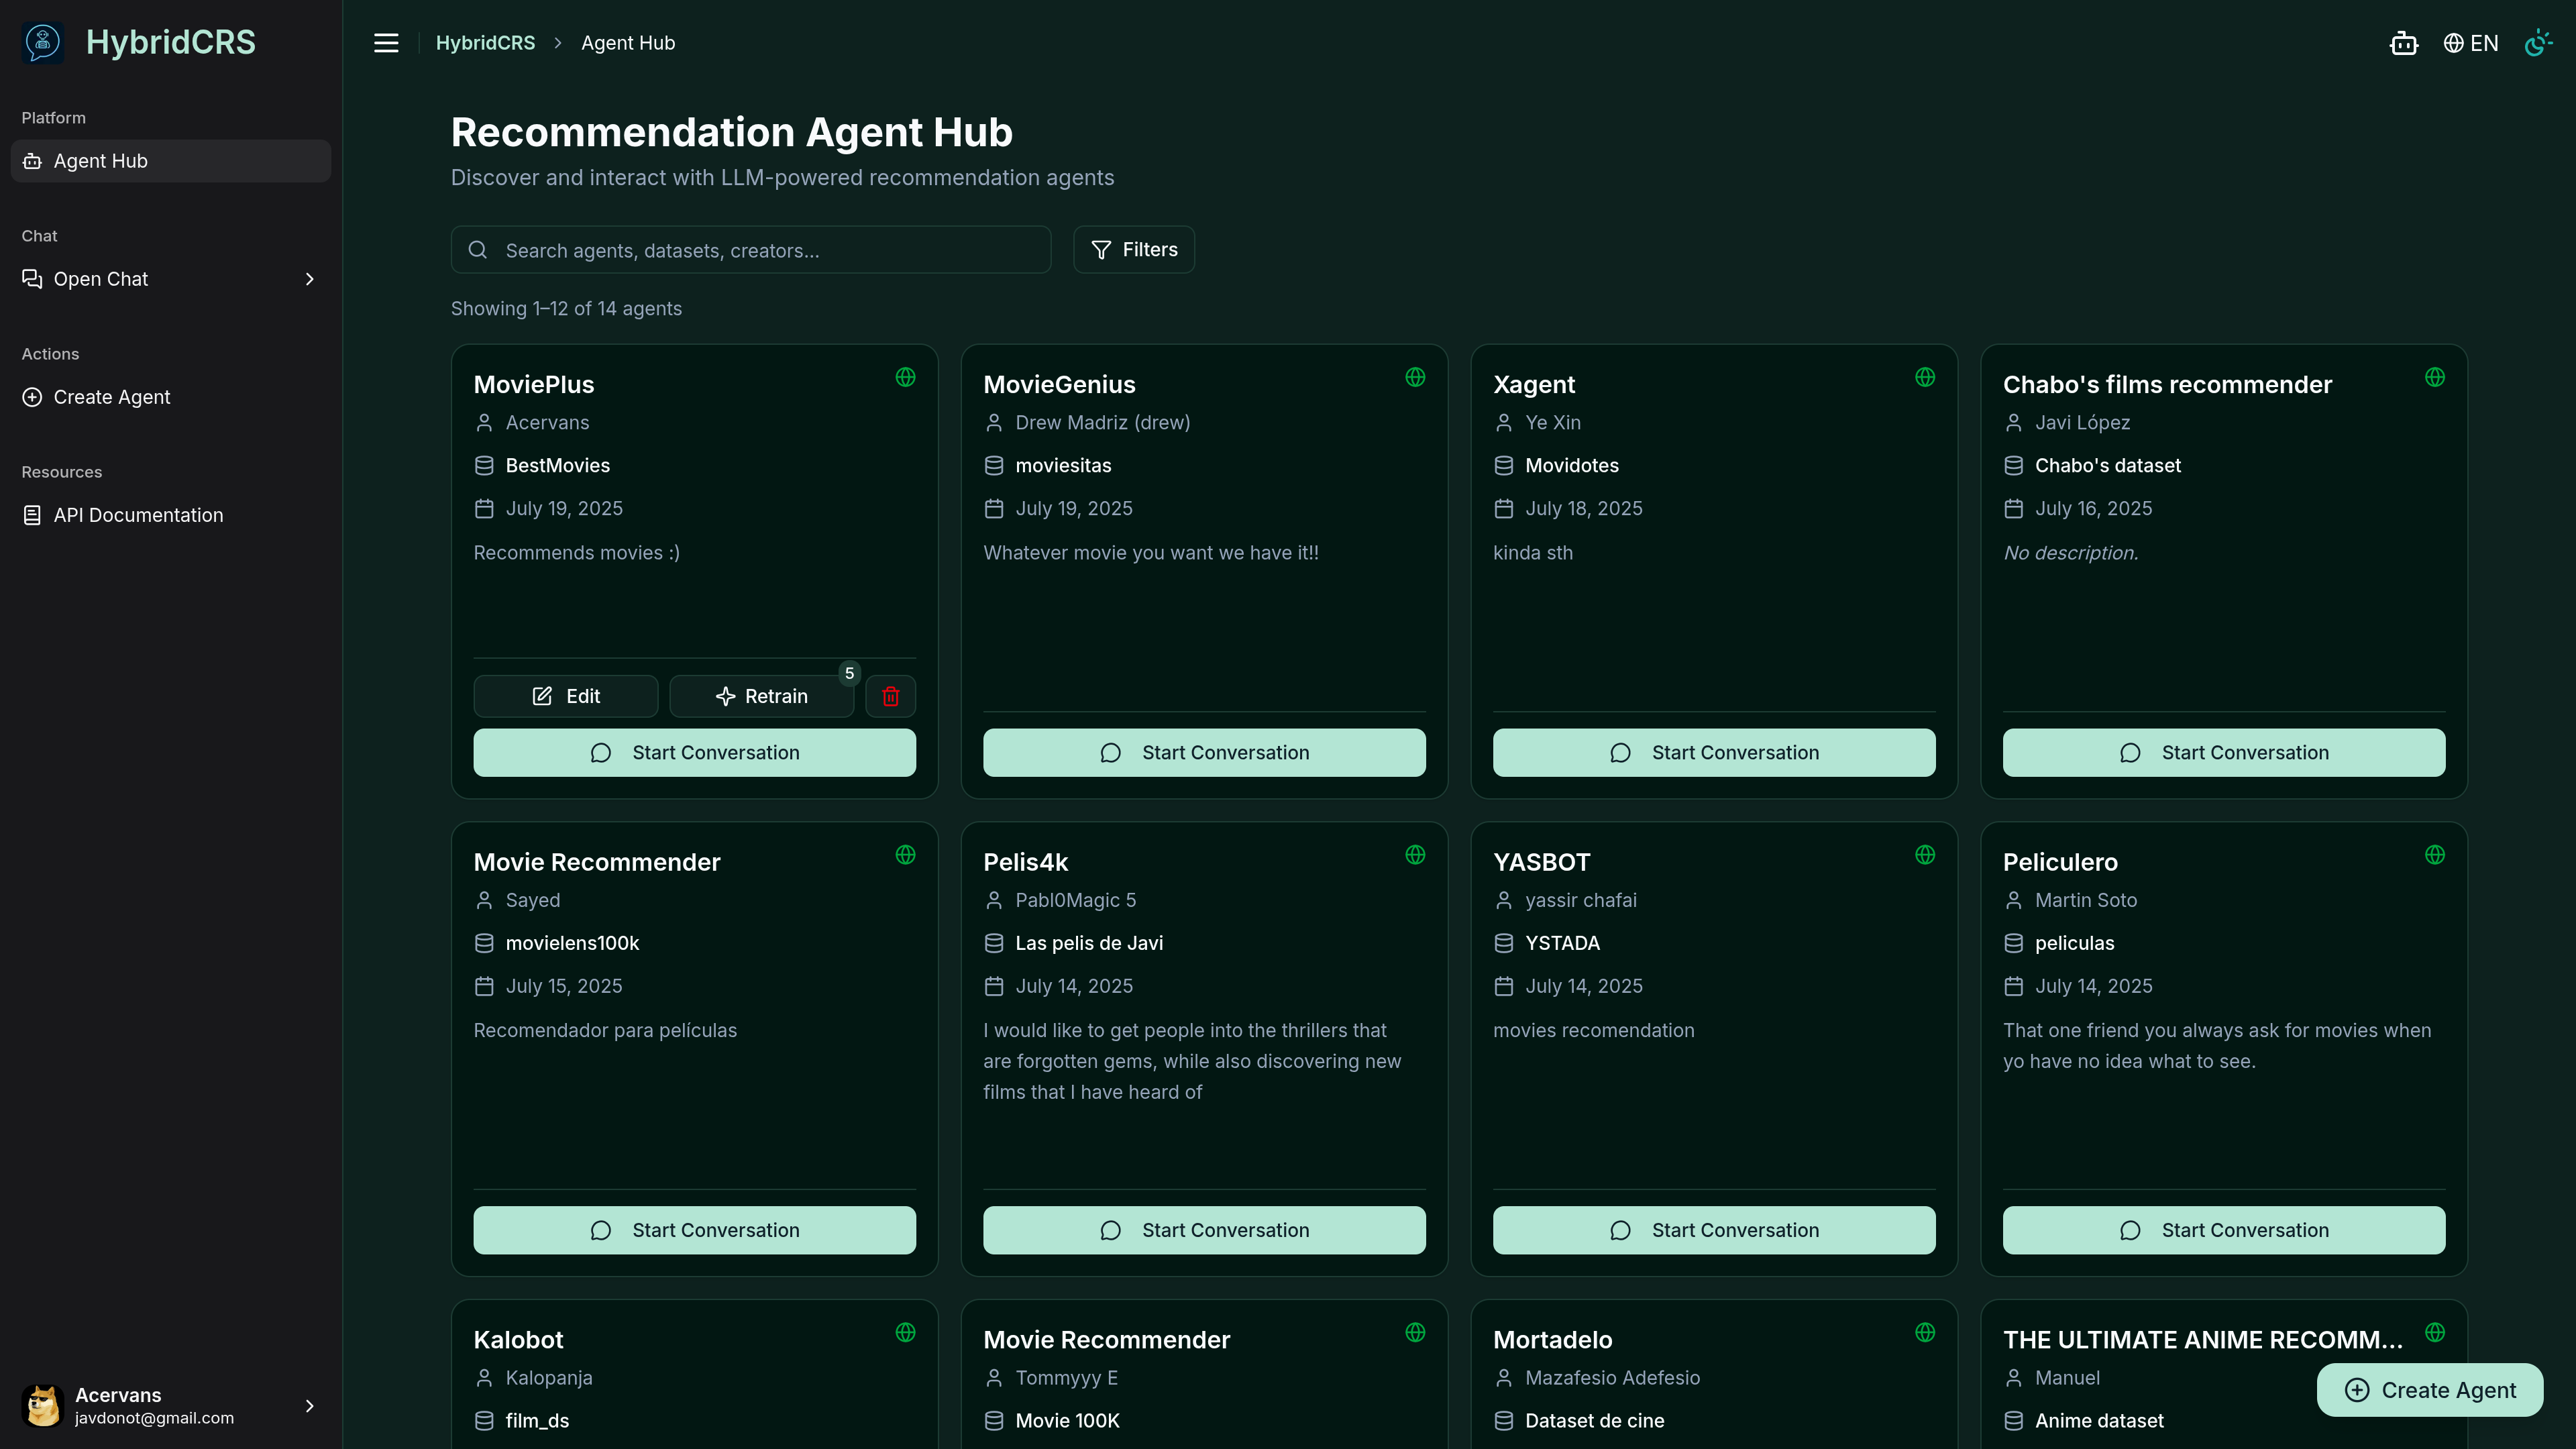
\includegraphics[width=\textwidth]{screenshots/agent_hub.png}
\end{figure}

For the conversational interfaces, the \texttt{@assistant-ui/react} library was of significant value. It provides a set of primitives specifically designed for building \acs{ai} chat applications. The \texttt{Thread} component leverages these primitives to create the entire chat experience, including the message list, the composer for user input, and action bars for interacting with messages. This results in a feature-rich and intuitive conversational interface, as illustrated in Figure~\ref{FIG:AGENT_CHAT} and Figure~\ref{FIG:OPEN_CHAT}. Particularly for the Agent Chat view, a custom component was developed to enhance the user experience for displaying recommendations, allowing the user to rate each recommended item with a rating slider, and sending the feedback to the backend as a JSON string.

\begin{figure}[Agent Chat]{FIG:AGENT_CHAT}{The main conversational interface for interacting with an agent.}
    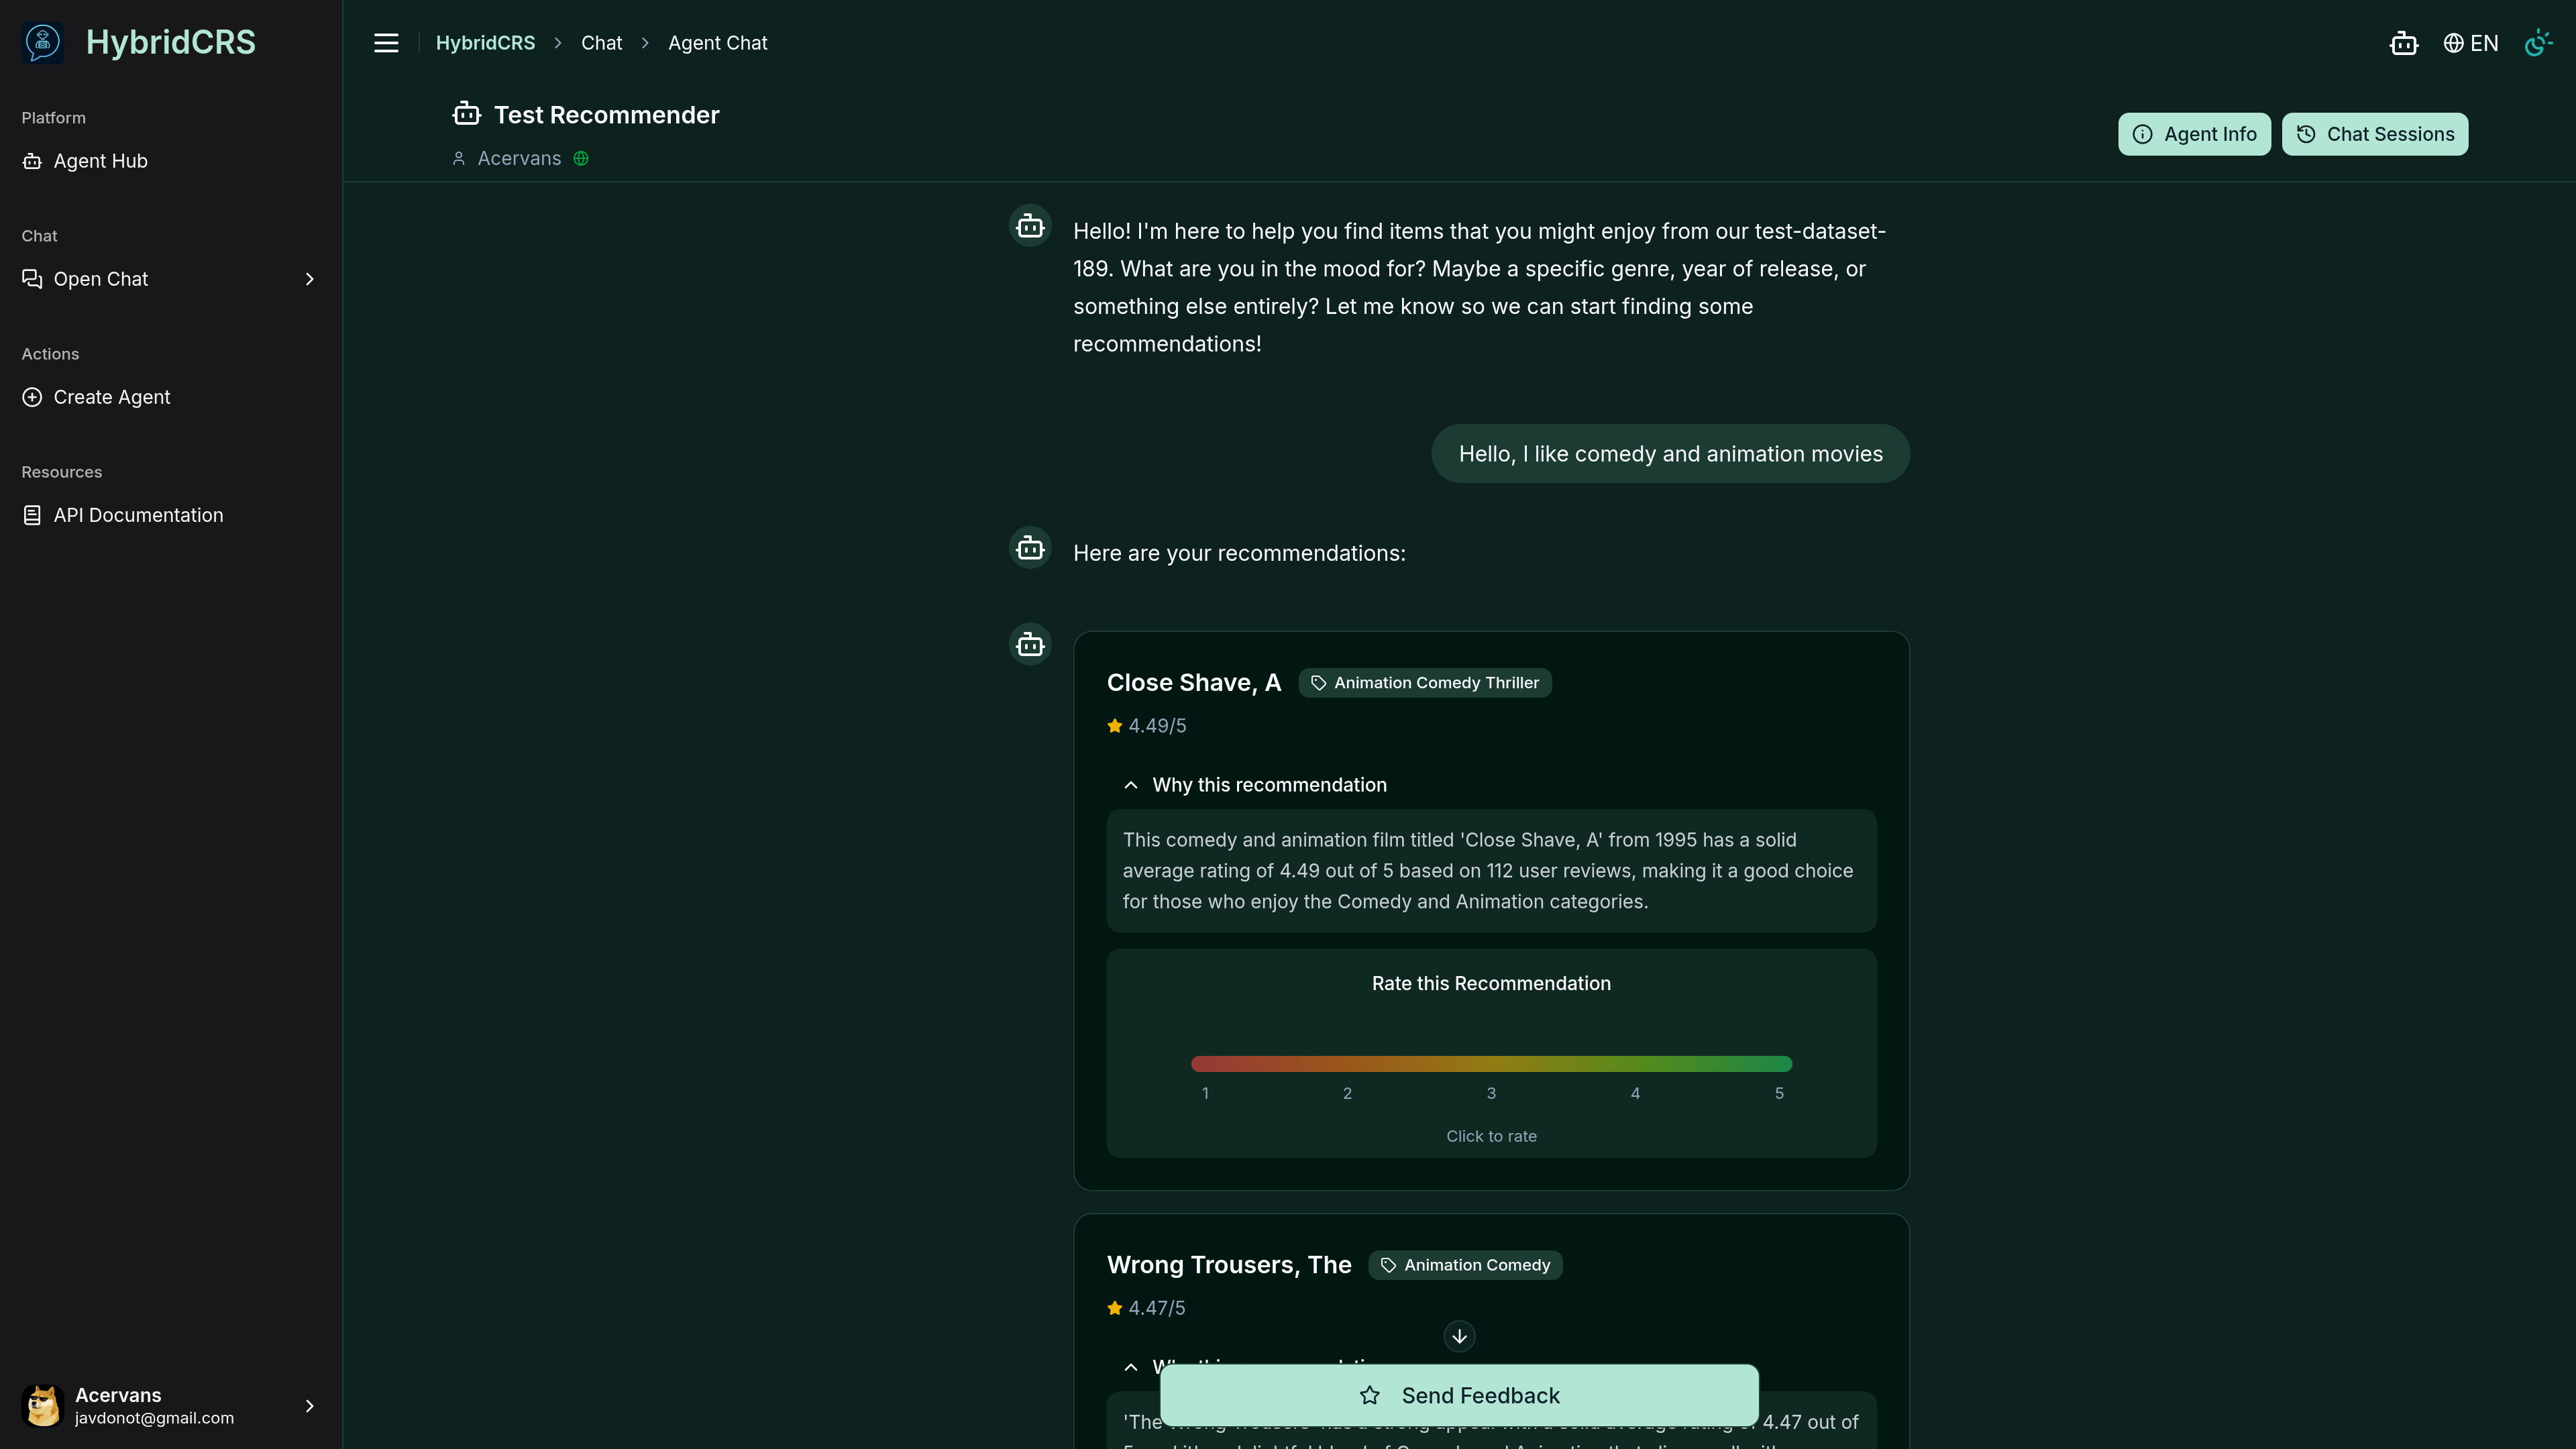
\includegraphics[width=\textwidth]{screenshots/agent_chat.png}
\end{figure}

\begin{figure}[Open Chat]{FIG:OPEN_CHAT}{The main conversational interface for open conversations with \acsp{llm}.}
    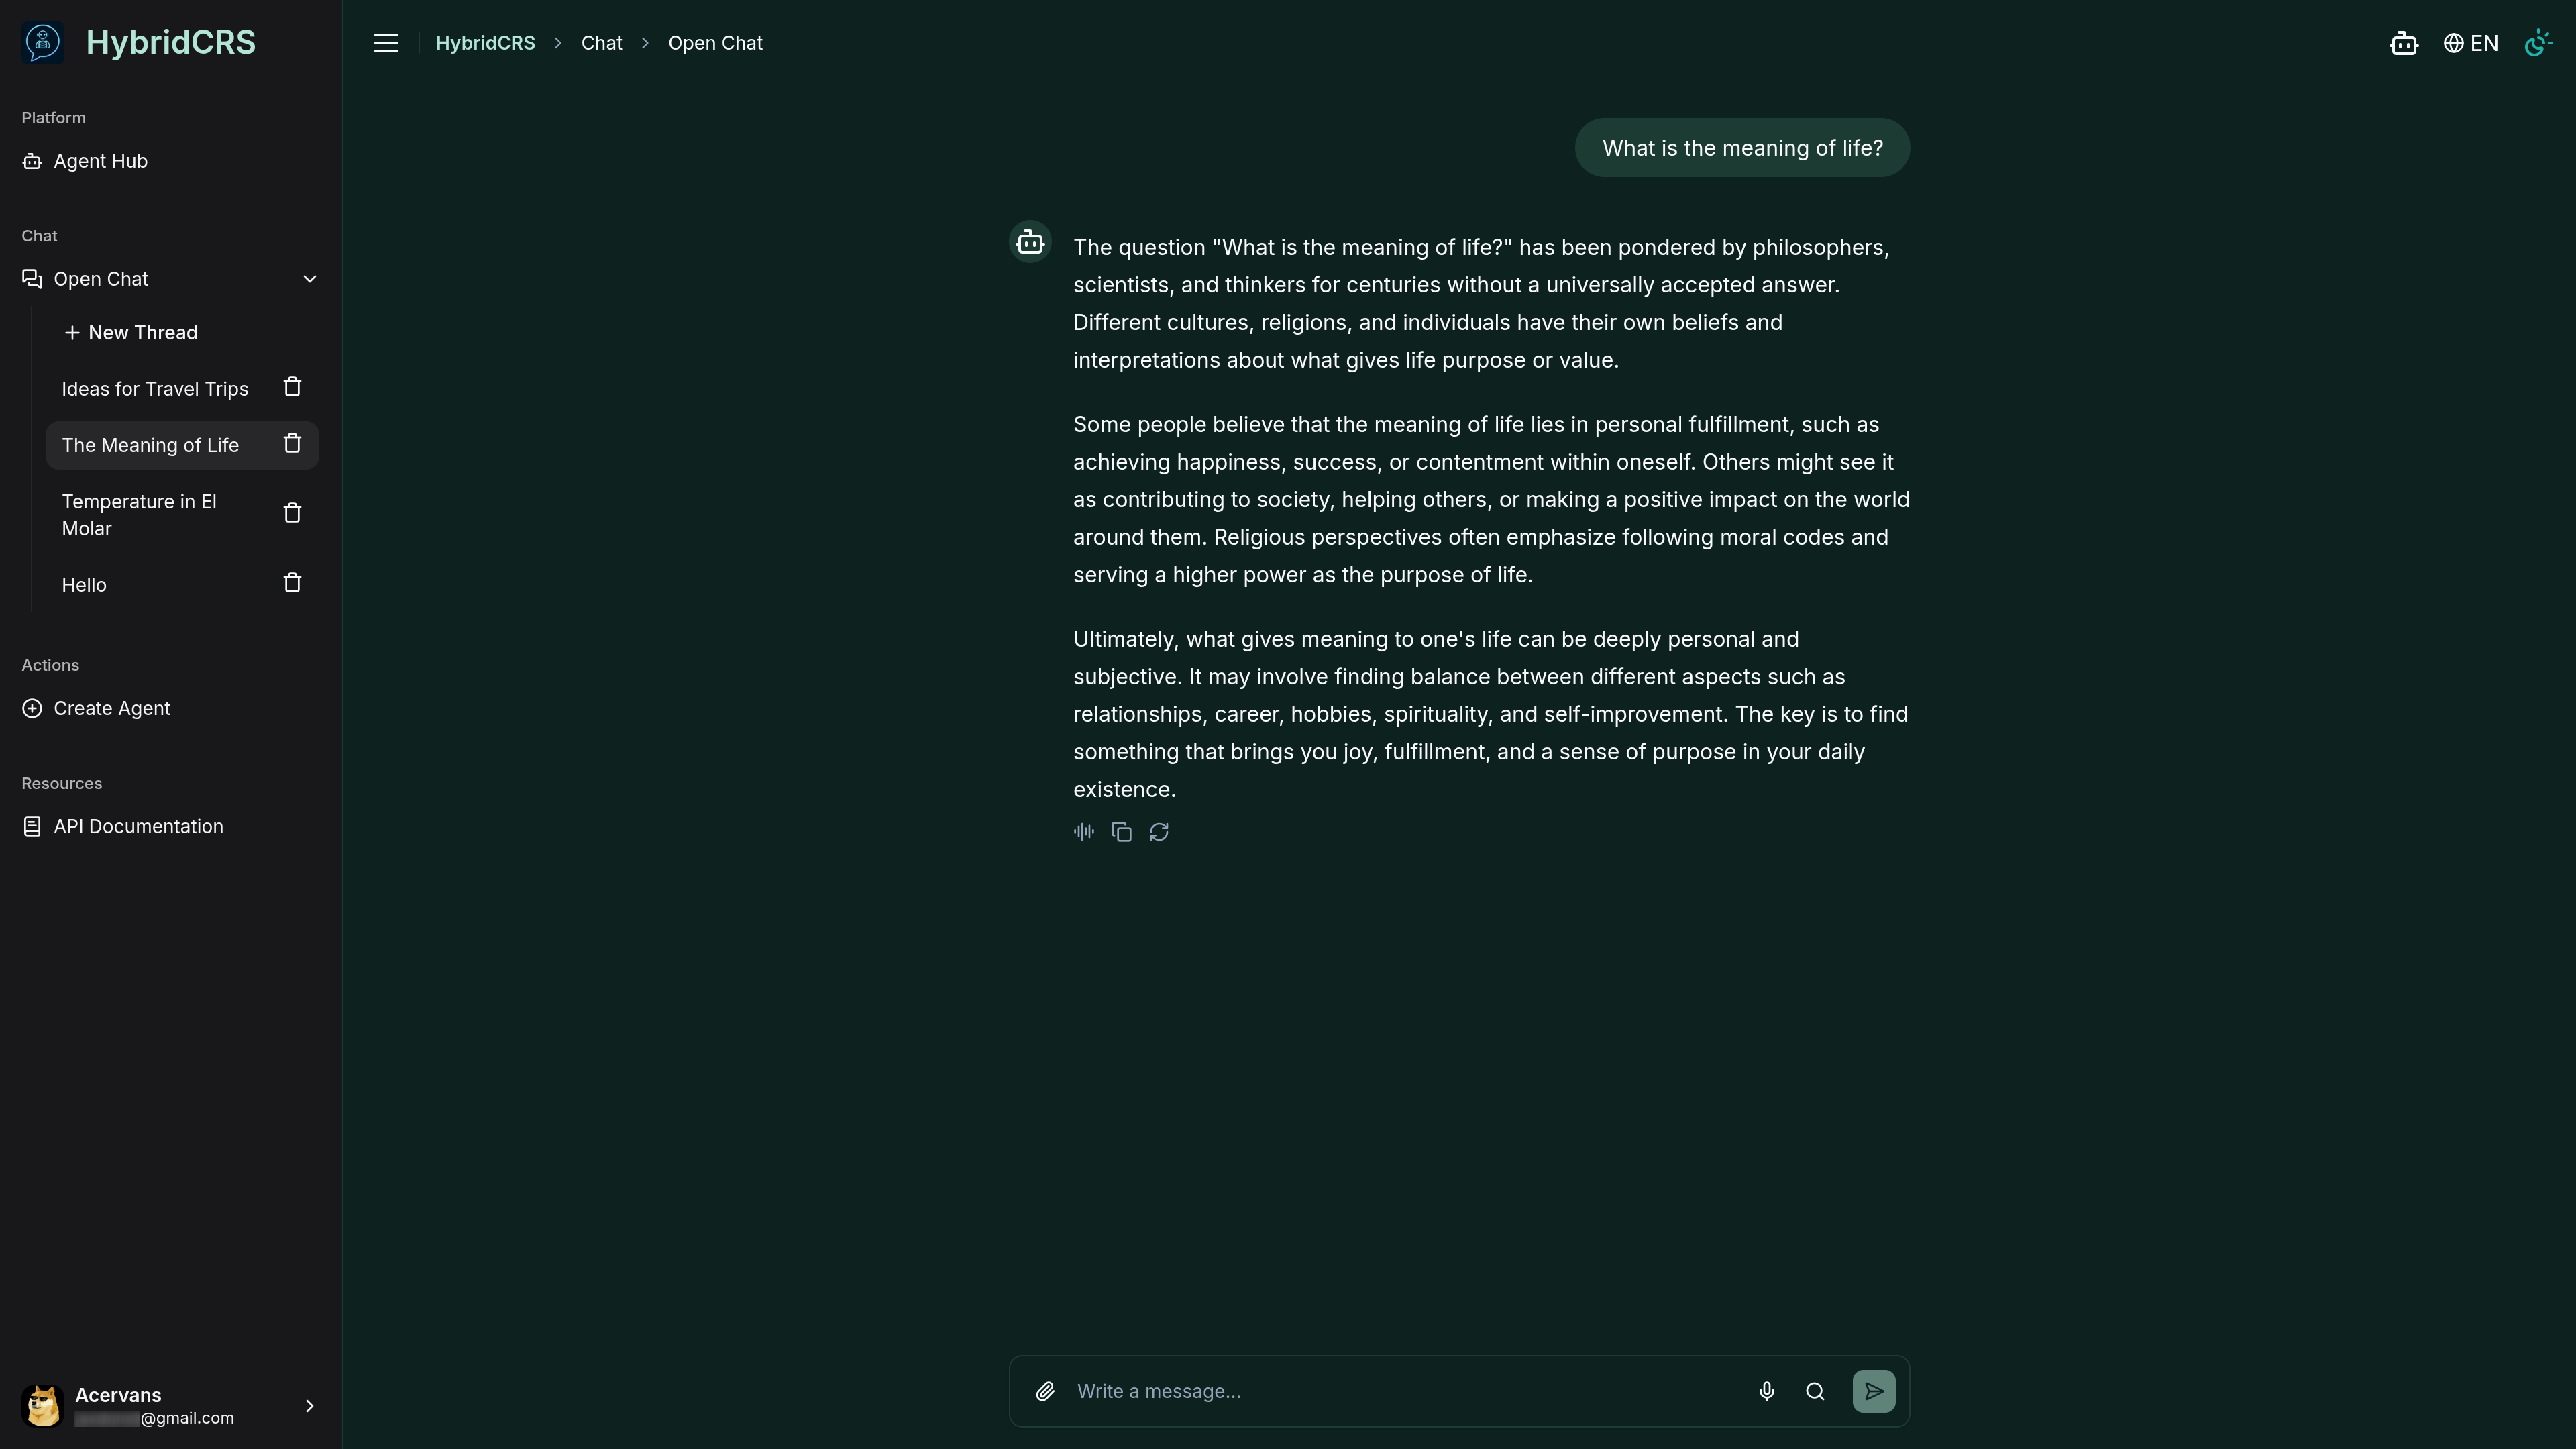
\includegraphics[width=\textwidth]{screenshots/open_chat.png}
\end{figure}

For the creation of agents, the \texttt{CreateAgent} view is designed to be user-friendly and intuitive, as displayed in Figure~\ref{FIG:CREATE_AGENT}. It guides users through the three steps, firstly to define an agent's name, dataset name and description; secondly to upload the datasets to be used for the graph and expert \aclp{rs}, with interactive previews of the data to configure the data type and column role of each column; and lastly to review and confirm the agent's configuration before creation.

\begin{figure}[Create Agent]{FIG:CREATE_AGENT}{Step one of the agent creation view.}
    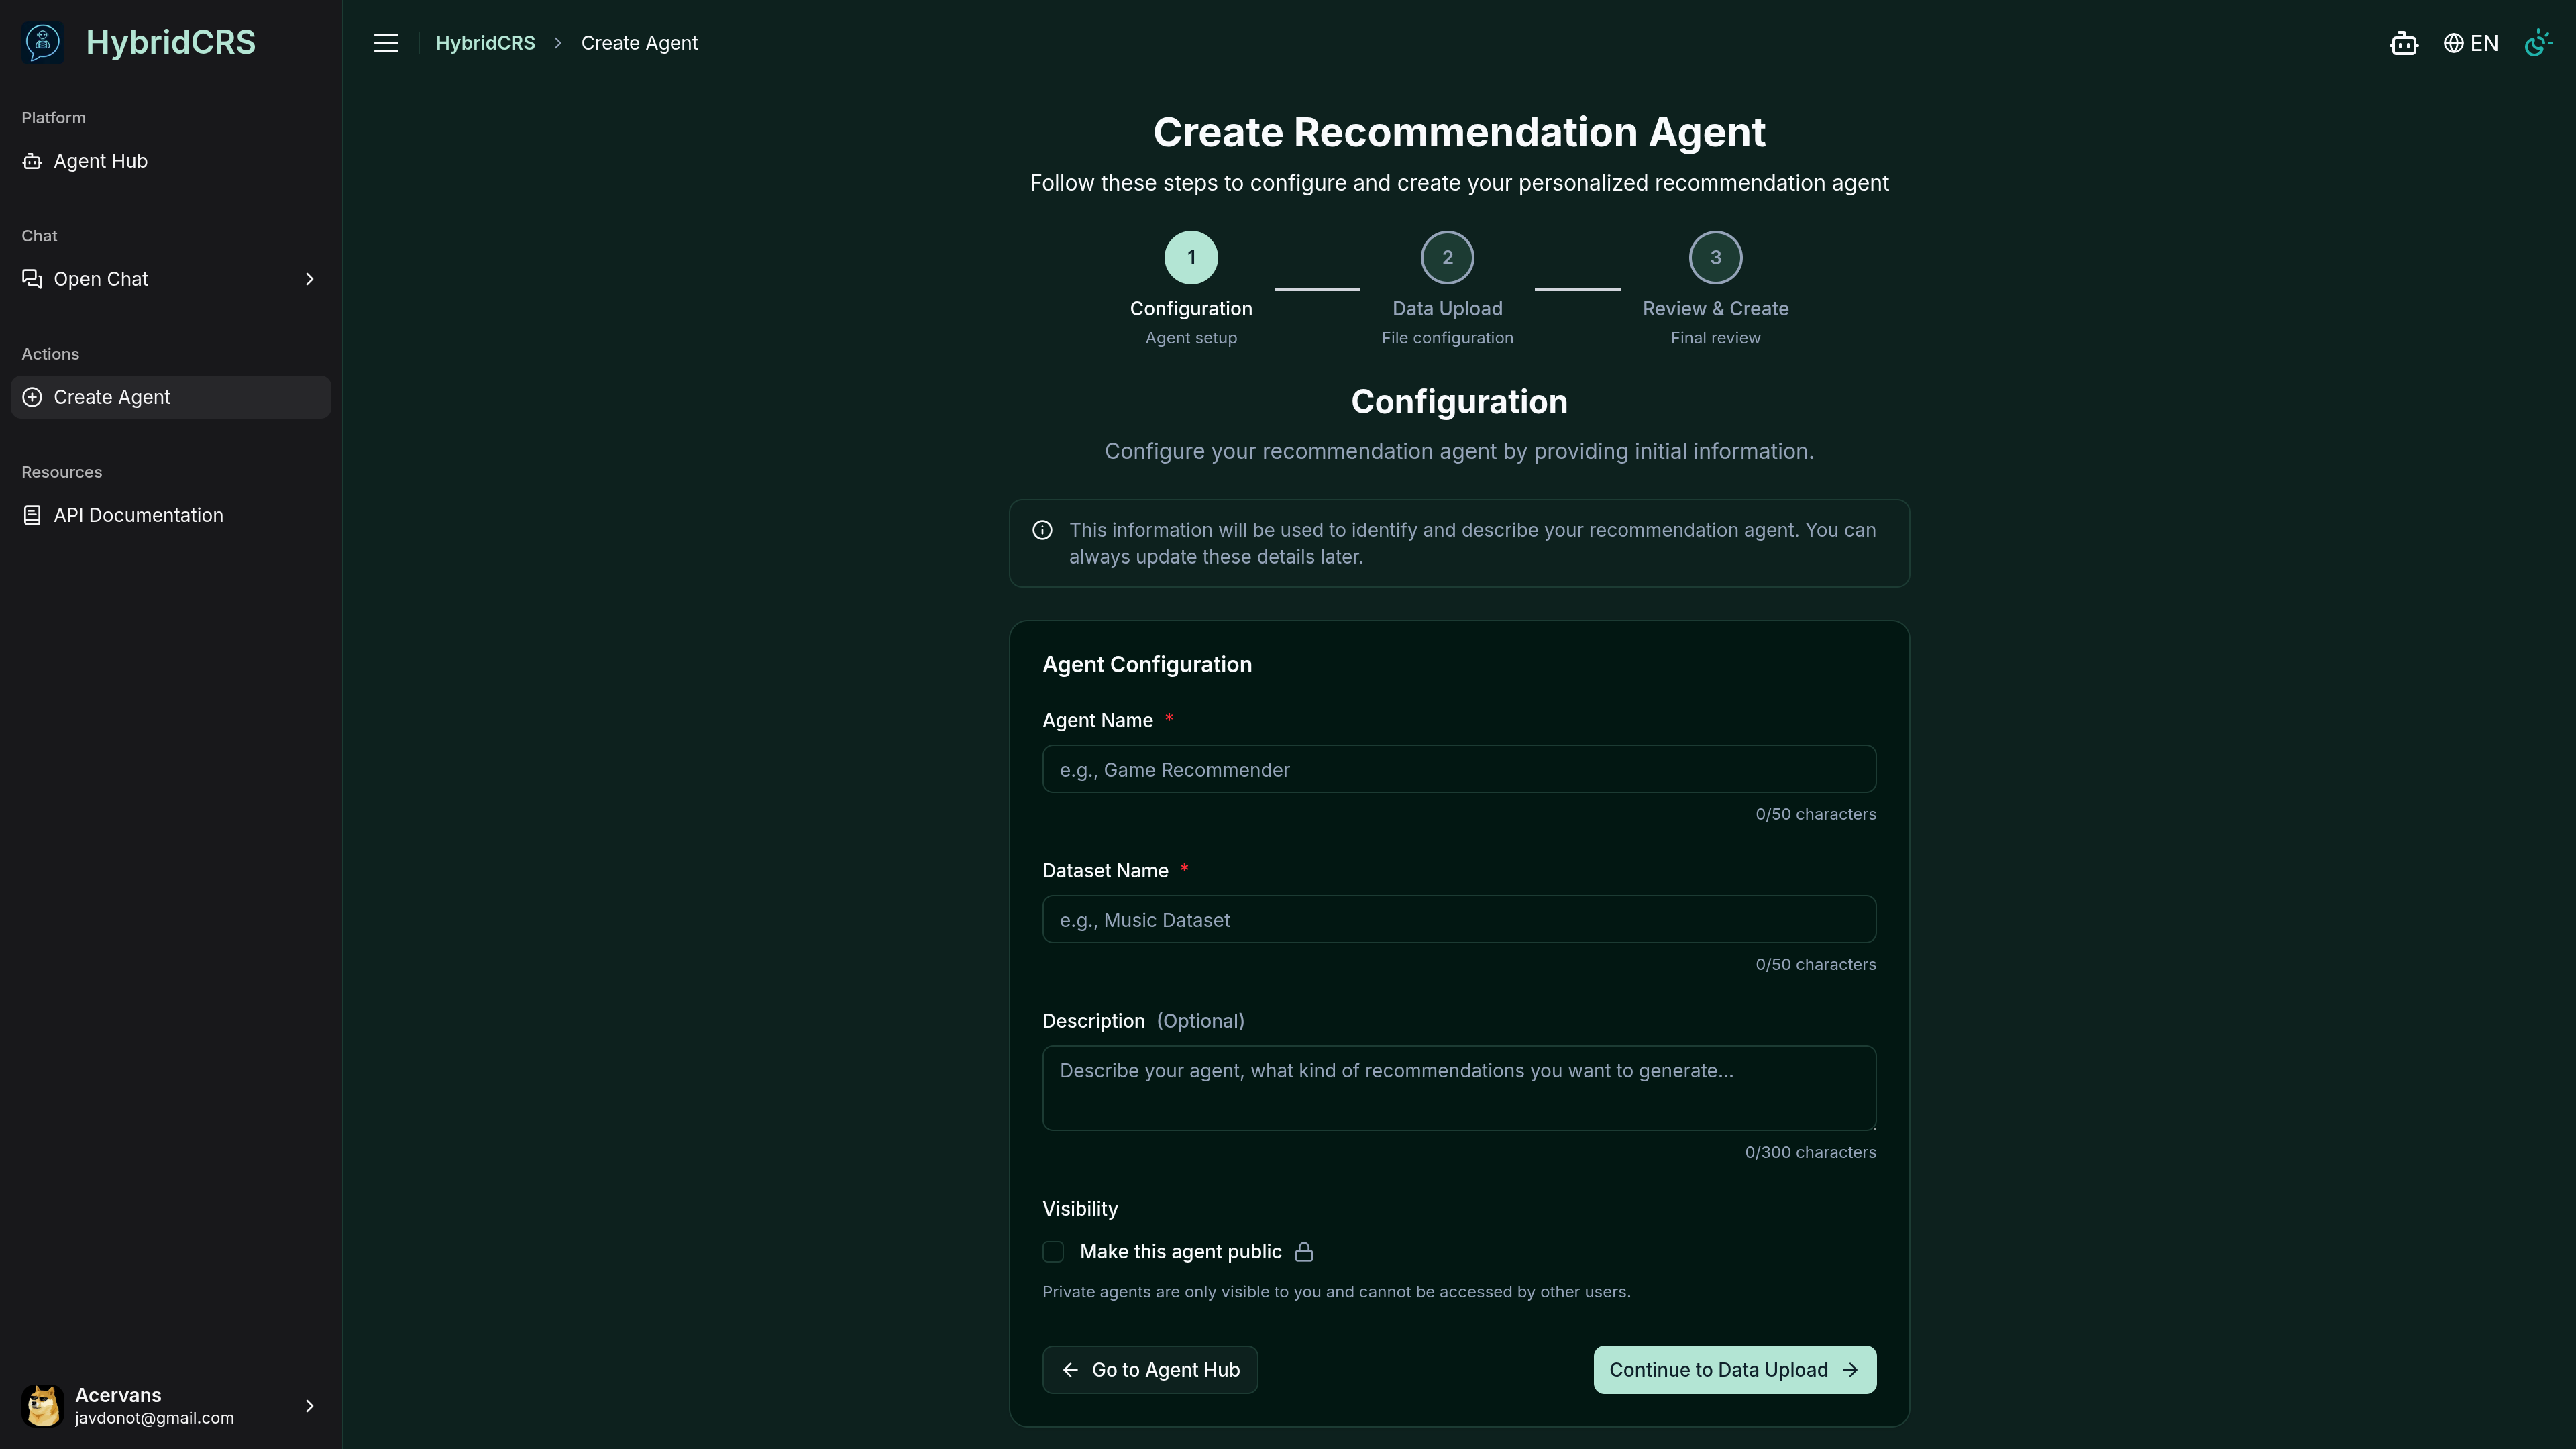
\includegraphics[width=\textwidth]{screenshots/create_agent_1.png}
\end{figure}

More views of the platform's user interface can be found in Appendix~\ref{AP:WEB_APP_SCREENSHOTS}, with mobile screenshots of the main views included in Appendix~\ref{AP:MOBILE_SCREENSHOTS} showcasing the \ac{pwa}'s responsive design.